% Created 2025-01-13 Mon 20:59
% Intended LaTeX compiler: pdflatex
\documentclass[presentation]{beamer}
\usepackage[utf8]{inputenc}
\usepackage[T1]{fontenc}
\usepackage{graphicx}
\usepackage{longtable}
\usepackage{wrapfig}
\usepackage{rotating}
\usepackage[normalem]{ulem}
\usepackage{amsmath}
\usepackage{amssymb}
\usepackage{capt-of}
\usepackage{hyperref}
\nocite{*}
\usepackage[T1]{fontenc}
\usepackage[utf8]{inputenc}
\usepackage[spanish]{babel}
\usepackage[backend=biber, style=apa]{biblatex}
\addbibresource{/home/davidmz/ArquitecturaGIT/bibliography.bib}
\usetheme{{Madrid}}
\usecolortheme{}
\usefonttheme{}
\useinnertheme{}
\useoutertheme{}
\author{Elizabeth Lopez, Francisco Morales, Juan Murillo , Angel Falcon, Danny Tipan, Anderson Herrera, Sebastian Chicaiza, Jairo Angulo}
\date{2025-01-13}
\title{S8-Buses-del-Sistema}

\hypersetup{
 pdfauthor={Elizabeth Lopez, Francisco Morales, Juan Murillo , Angel Falcon, Danny Tipan, Anderson Herrera, Sebastian Chicaiza, Jairo Angulo},
 pdftitle={S8-Buses-del-Sistema},
 pdfkeywords={},
 pdfsubject={},
 pdfcreator={Emacs 27.1 (Org mode 9.3)}, 
 pdflang={Spanish}}
\begin{document}

\maketitle
\begin{frame}{Outline}
\tableofcontents
\end{frame}



\section{Buses del Sistema (Sección)}
\label{sec:org274efe4}
\begin{frame}[label={sec:org17f1210}]{Estructuras de Interconexión (E1, 7, 97)}
\begin{itemize}
\item Conjunto de líneas que conectan los módulos elementales de un computador.
Para que se comuniquen e intercambien datos.
\item La estructura depende de los intercambios que se produzcan en los módulos.
\end{itemize}

\begin{center}
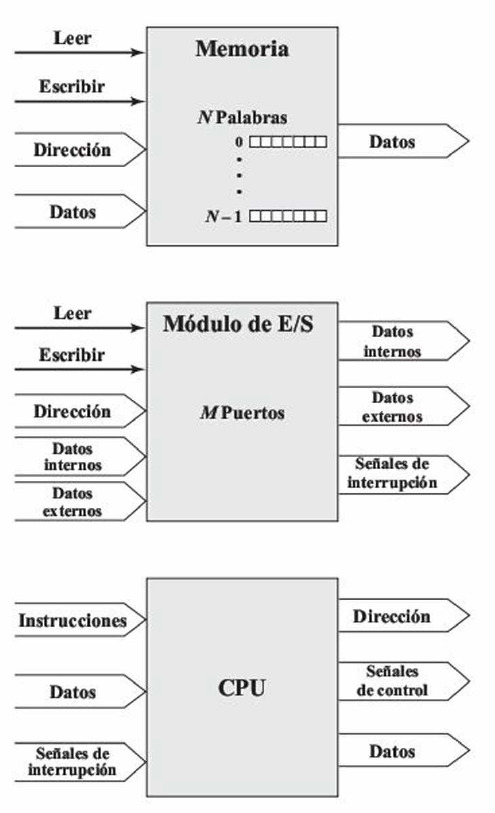
\includegraphics[width=0.3\textwidth]{./Images/Modulos.jpg}
\end{center}
\end{frame}

\begin{frame}[label={sec:orgbab70de}]{Estructuras de Interconexión (E1, 7, 97)}
\alert{Módulos:}

\begin{itemize}
\item \alert{\alert{Memoria:}} constituido por N palabras de igual longitud. Se pueden realizar las
operaciones Read(Leer) y Write(Escribir). La posición de memoria se especifica
mediante una dirección.
\item \alert{\alert{Módulo de E/S:}} se encarga de controlar los dispositivos externos enlazados
a los puertos, donde se les asignara una dirección M. Controla los datos de salida
y entrada. Realiza las operaciones de lectura y escritura. Envía señales de interrupción.
\item \alert{\alert{Procesador:}} lee instrucciones y datos. Escribe datos después de procesarlos y
controla el funcionamiento del sistema. Puede recibir señales de interrupción.
\end{itemize}
\end{frame}

\begin{frame}[label={sec:orga276795}]{Estructuras de Interconexión (E1, 7, 97)}
\alert{Intercambios de Datos:}

\begin{itemize}
\item \alert{\alert{Memoria a procesador:}} el procesador lee información desde la memoria.
\item \alert{\alert{Procesador a memoria:}} el procesador escribe un dato en la memoria.
\item \alert{\alert{E/S a procesador:}} el procesador lee datos de un dispositivo de E/S.
\item \alert{\alert{Procesador a E/S:}} el procesador envía datos al dispositivo de  E/S.
\item \alert{\alert{Memoria a E/S - E/S a Memoria:}} ambos intercambian datos directamente.
\end{itemize}
\end{frame}

\section{Interconexión con Buses (Sección)}
\label{sec:org54dce4a}
\begin{frame}[label={sec:org57fb148}]{Interconexión con Buses (E1, 7, 99)}
\begin{itemize}
\item Los buses son caminos de comunicación entre dos o más dispositivos con la
habilidad de transmitir señales hacia los demás o recibir las señales emitidas.
\item Solo un dispositivo puede emitir la señal en un periodo de tiempo. Si ambos
transmiten la señal, esta podria solaparse y distorsionarse.
\item Los caminos o lineas del bus transmiten señales binarias ya sea a travez de una
sola línea o de varias de manera paralela.
\item Existen diferentes tipos de buses para la comunicacion de diversos componentes.
El que trabaja con los módulos elementales se denomina (System bus).
\end{itemize}
\end{frame}

\begin{frame}[label={sec:org2a6b81d}]{Estructura del Bus  (E1, 7, 99)}
\begin{center}
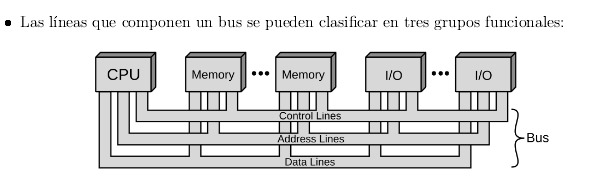
\includegraphics[width=0.8\textwidth]{./Images/Lineas.jpg}
\end{center}

\begin{itemize}
\item ¿Qué tipos de líneas componen un Bus de Sistema?
\begin{itemize}
\item Lineas de datos.
\item Lineas de direccion.
\item Lineas de control.
\end{itemize}
\end{itemize}
\end{frame}

\begin{frame}[label={sec:orga6f5b8d}]{Estructura del Bus}
\begin{itemize}
\item ¿Qué son las líneas de datos?
\begin{itemize}
\item Transporte
\item Datos
\item Memoria -> Procesador
\end{itemize}
\end{itemize}
\end{frame}

\begin{frame}[label={sec:orgce4d684}]{Estructura del Bus}
\begin{itemize}
\item ¿Qué son las líneas de dirección?
\begin{itemize}
\item Ubicación
\item Memoria
\item Puertos de E/S
\item Anchura del bus
\end{itemize}
\end{itemize}
\end{frame}

\begin{frame}[label={sec:org91f8d5a}]{Estructura del Bus}
\begin{itemize}
\item ¿Qué son las líneas de control?
\begin{itemize}
\item Control
\item Señales
\item Escritura
\item Lectura
\end{itemize}
\end{itemize}
\end{frame}

\begin{frame}[label={sec:orgef98df3}]{Jerarquía de Buses Múltiples (E2, 7)}
Si se conecta un gran número de dispositivos al bus, las prestaciones pueden disminuir. Hay dos causas principales: 

\begin{enumerate}
\item Mayor retarde de propagación. Este retardo determina el tiempo que necesitan los dispositivos para coordinarse en el uso del bus.

\item Posible cuello de botella. Este problema se puede resolver en alguna medida incrementando la velocidad a la que el bus puede transferir los datos y utilizando buses más anchos (por ejemplo incrementando el bus de datos de 32 a 64 bits)
\end{enumerate}
\end{frame}
\begin{frame}[label={sec:orge9058df}]{Jerarquía de buses múltiples}
Por consiguiente, la mayoría de los computadores utilizan varios buses, normalmente organizados
jerárquicamente.

\begin{center}
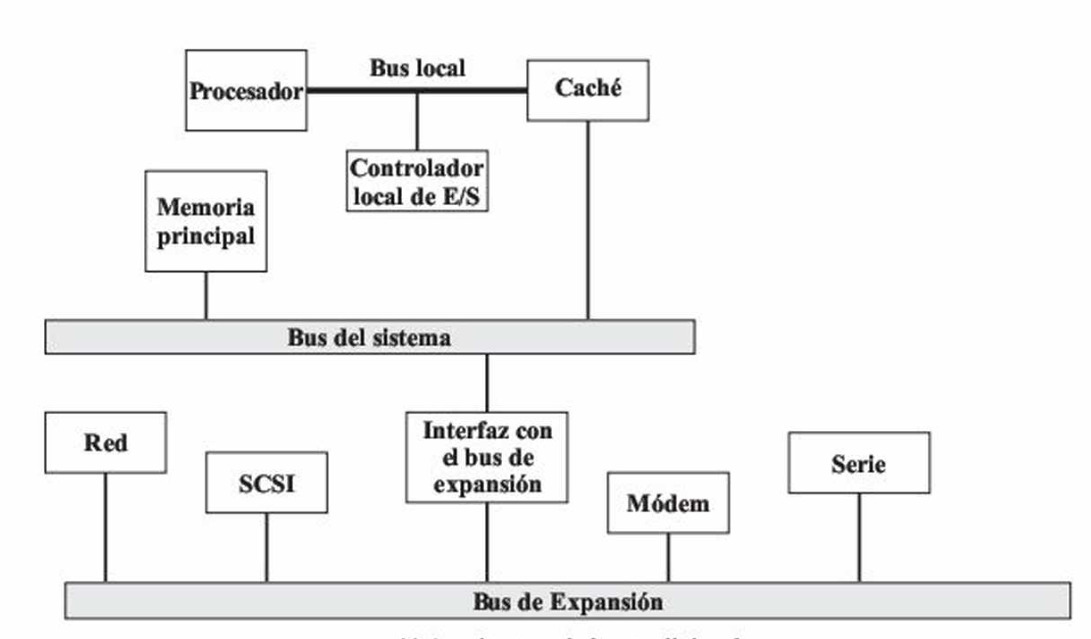
\includegraphics[width=0.8\textwidth]{./Images/jerarquiaBuses.jpeg}
\end{center} 
\end{frame}
\begin{frame}[label={sec:org3ed469a}]{Jerarquía de buses múltiples}
La respuesta común a esta
situación, por parte de la industria, ha sido proponer un bus de alta velocidad que está estrechamente
integrado con el resto del sistema, y requiere solo un adaptador (bridge) entre el bus del procesador y
el bus de alta velocidad. En algunas ocasiones, esta disposición es conocida como arquitectura de
entreplanta (mezzanine architecture).

\begin{center}
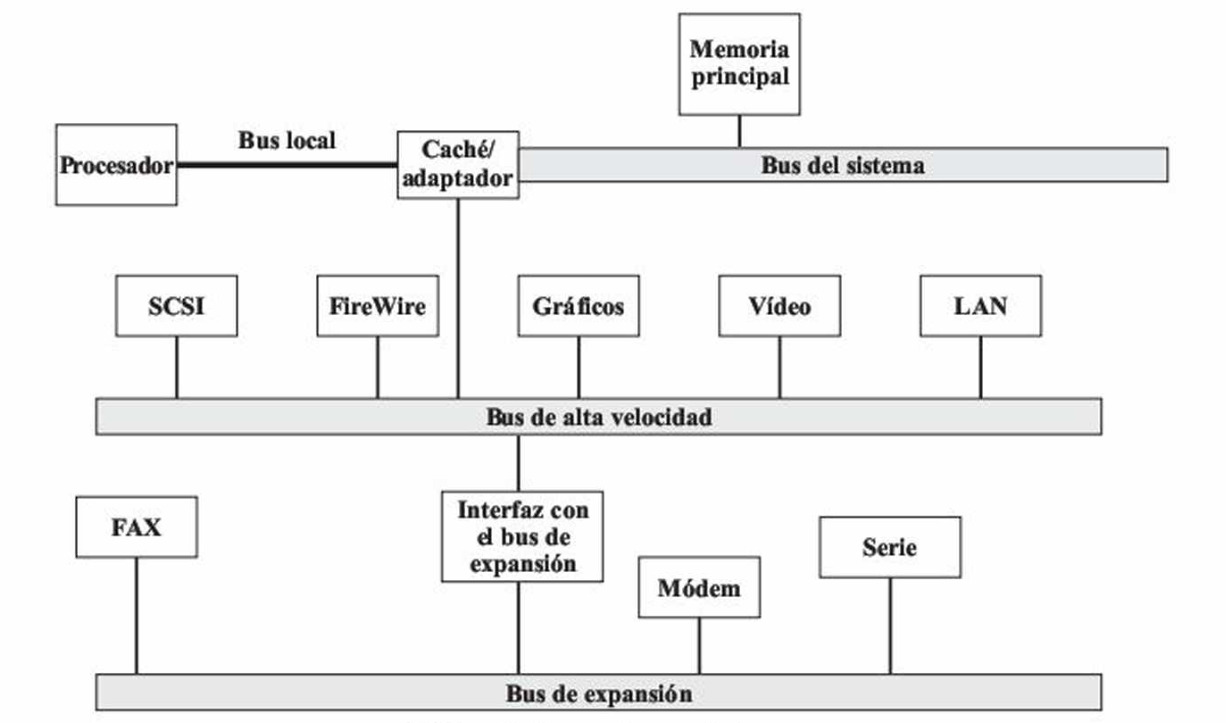
\includegraphics[width=0.8\textwidth]{./Images/jerarquiaBuses2.jpeg}
\end{center}
\end{frame}

\begin{frame}[label={sec:org7d4c6f6}]{Jerarquía de buses múltiples}
La ventaja de esta organización es que el bus de alta velocidad acerca al procesador los dispositi
vos que exigen prestaciones elevadas y al mismo tiempo es independiente del procesador. Así, se pue
den tolerar las diferencias de velocidad entre el procesador y el bus de altas prestaciones y las
variaciones en la definición de las líneas de los buses. Los cambios en la arquitectura del procesador
no afectan al bus de alta velocidad, y viceversa.
\end{frame}
\begin{frame}[label={sec:org569936d}]{Elementos de Diseño de un Bus (E2, 7)}
\end{frame}
\section{Buses del Sistema (Sección)}
\label{sec:org53cd128}

\begin{center}
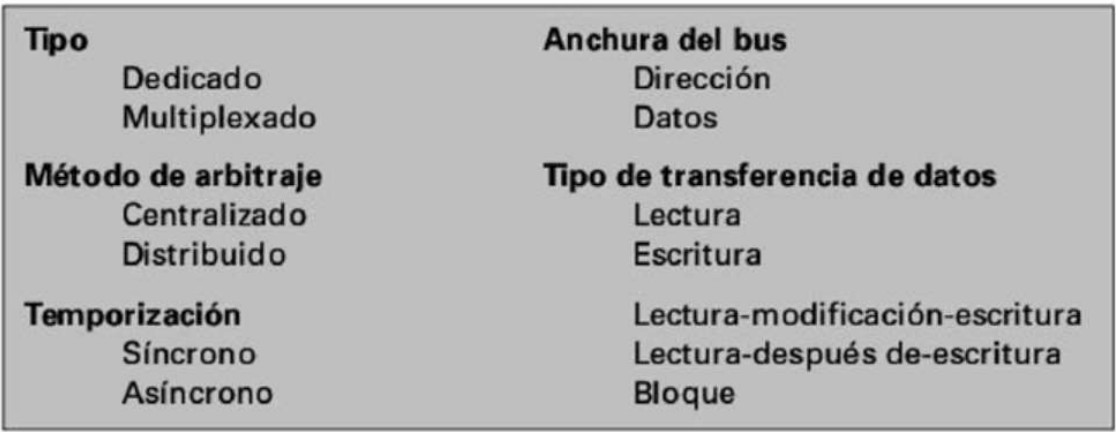
\includegraphics[width=0.8\textwidth]{./Images/bus.jpg}
\end{center}

\begin{frame}[label={sec:orgeaf39b9}]{Elementos de Diseño de un Bus (E2, 7)}
\begin{block}{1. Tipo}
\begin{itemize}
\item \alert{Dedicado}: El bus está reservado para una única función o dispositivo, asegurando una comunicación directa y sin interferencias.
\item \alert{Multiplexado}: Se comparte el mismo bus para diferentes tipos de datos o señales (por ejemplo, datos y direcciones), utilizando mecanismos de temporización o control para alternar entre usos.
\end{itemize}
\end{block}



\begin{block}{2. Método de arbitraje}
\begin{itemize}
\item \alert{Centralizado}: Existe un único controlador que decide cuál dispositivo puede usar el bus en cada momento. Es más sencillo de implementar pero puede ser un punto único de fallo.
\item \alert{Distribuido}: La responsabilidad del control del bus se reparte entre los dispositivos conectados, permitiendo un diseño más robusto y descentralizado.
\end{itemize}
\end{block}
\end{frame}
\begin{frame}[label={sec:orgdf46091}]{Elementos de Diseño de un Bus (E2, 7)}
\begin{block}{3. Temporización}
\begin{itemize}
\item \alert{Síncrono}: Las transferencias de datos se realizan basándose en un reloj común. Es más rápido, pero menos flexible, ya que todos los dispositivos deben funcionar a la misma velocidad.
\item \alert{Asíncrono}: No requiere un reloj común, permitiendo que cada dispositivo opere a su propia velocidad. Es más flexible, aunque más complejo de coordinar.
\end{itemize}
\end{block}



\begin{block}{4. Anchura del bus}
\begin{itemize}
\item \alert{Dirección}: Define el número de líneas disponibles para las direcciones, lo que determina la cantidad máxima de dispositivos o memoria que se pueden direccionar.
\item \alert{Datos}: Indica el número de bits que se pueden transferir simultáneamente, influyendo en la velocidad del sistema (por ejemplo, un bus de datos de 32 bits permite transferir 32 bits en paralelo).
\end{itemize}
\end{block}
\end{frame}

\begin{frame}[label={sec:orgeac6e69}]{Elementos de Diseño de un Bus (E2, 7)}
\begin{block}{5. Tipo de transferencia de datos}
\begin{itemize}
\item \alert{Lectura}: Se transfieren datos desde un dispositivo (por ejemplo, memoria) al bus para que sean utilizados por otro dispositivo.
\item \alert{Escritura}: Se envían datos desde un dispositivo al bus para almacenarlos en otro (como en memoria).
\item \alert{Lectura-modificación-escritura}: Un ciclo donde se lee un dato, se modifica y luego se escribe de nuevo en memoria o dispositivo.
\item \alert{Lectura-después-de-escritura}: Se escriben los datos en un dispositivo y luego se leen para verificar la operación.
\item \alert{Bloque}: Se transfieren varios datos consecutivos en una sola operación, optimizando la eficiencia para grandes volúmenes de datos.
\end{itemize}
\end{block}
\end{frame}


\section{Interconexión punto a punto}
\label{sec:org8b97689}
\begin{frame}[label={sec:orgffe67cd}]{Interconexión punto a punto}
La interconexión punto a punto consiste en establecer una conexión directa entre dos componentes de un sistema informáticos.
Esta arquitectura reemplazo a los buses compartidos, y la principal razón fue el aumento de frecuencia.

\begin{figure}[!h]
   \vspace{-0.1cm}
   \centering
   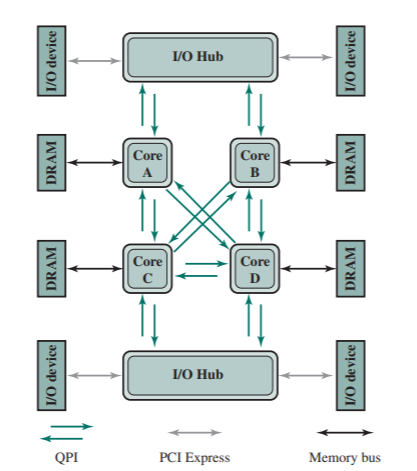
\includegraphics[height=4cm, width=0.8\textwidth]{./Images/image1.png}
   \vspace{-0.5cm} % Ajusta el espacio inferior
   \caption{Multiprocesador con QPIs}
   \label{fig:Representacion}
\end{figure}
\end{frame}

\begin{frame}[label={sec:org2fdf55a}]{Ventajas}
\begin{columns}
\begin{column}{0.8\columnwidth}
\begin{itemize}
\item Elimina cuellos de botella asociados con buses compartidos.
\item Mejora la escalabilidad en sistemas multiprocesador, ya que cada procesador puede comunicarse con otros sin interferencias.
\item Aumenta la velocidad de transferencia y reduce la latencia.
\end{itemize}
\end{column}
\end{columns}
\end{frame}
\section{Introducción QPI}
\label{sec:org952d437}
\begin{frame}[label={sec:org626b543}]{Introducción QPI}
Fue creado para solucionar los problemas de los buses compartidos, ofreciendo una conexión directa
y eficiente entre los componentes. Este tipo de interconexión mejora el rendimiento al permitir
una comunicación más rápida y efectiva entre los procesadores y otros dispositivos, sin las
restricciones de los buses. 
\par
\end{frame}
\begin{frame}[label={sec:orgbce7359}]{Características QPI:}
\begin{itemize}
\item Múltiples conexiones directas
\item Arquitectura de protocolo en capas
\item Transferencia de datos en paquetes
\end{itemize}
\end{frame}

\section{QuickPath Interconnect (QPI)}
\label{sec:org5d9216e}

\begin{frame}[label={sec:org3f658f2}]{Características de QPI}
\begin{itemize}
\item \alert{\alert{Múltiples conexiones directas:}}
\begin{itemize}
\item Cada componente (como el procesador, la memoria o los dispositivos de entrada/salida) se conecta
directamente con otros componentes de manera individual, sin tener que compartir el mismo canal.
\item Al tener conexiones directas, cada componente puede enviar y recibir datos sin esperar turno,
lo que hace que todo funcione de manera más rápida y eficiente.
\end{itemize}
\item \alert{\alert{Arquitectura de protocolo en capas:}}
\begin{itemize}
\item Se usan protocolos como TCP/IP para organizar y manejar la comunicación. En lugar de enviar
un mensaje de una sola forma simple, se utilizan diferentes pasos o etapas para asegurar que el
mensaje llegue correctamente.
\end{itemize}
\item \alert{\alert{Transferencia en paquetes:}}
\begin{itemize}
\item Los datos no se envían de manera continua, sino que se dividen en paquetes.
\item Cada paquete contiene una parte de los datos y también incluye información adicional, como encabezados
de control para saber a dónde deben ir los datos y códigos de control de errores para asegurarse de que
los datos no se pierdan o se dañen durante el envío.
\end{itemize}
\end{itemize}
\end{frame}


\begin{frame}[label={sec:org6edac9c}]{QPI una arquitectura de protocolo de cuatro capas}
\begin{center}
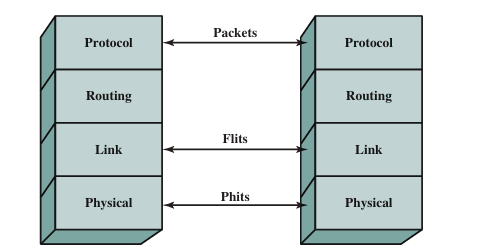
\includegraphics[width=.9\linewidth]{./Images/QPI.png}
\end{center}    
\end{frame}


\begin{frame}[label={sec:org723b50a}]{Arquitectura de protocolo QPI}
\begin{itemize}
\item \alert{\alert{Capa física:}}
\begin{itemize}
\item Está formada por 84 enlaces individuales, cada camino de datos consta de un par de cables,
llamados "carriles", que transmiten un bit a la vez.
\item Hay 20 carriles en cada dirección: una para enviar datos y otra para recibir.
\item Cada conjunto de 20 bits que se transmite se llama "phit", con una velocidad de transferencia
de 6.4 giga transferencias por segundo (GT/s).
\end{itemize}
\item \alert{\alert{Capa de enlace:}}
\begin{itemize}
\item Realiza dos funciones clave: control de flujo y control de errores.
Estas se aplican a cada "flit" (unidad de control de flujo).
\item Cada flit tiene una carga útil de 72 bits, que contiene los datos o mensajes.
\item Los flits de datos transportan los bits reales entre los procesadores y el
controlador de entrada/salida.
\item Los flits de mensaje se utilizan para funciones como el control de flujo y
el control de errores.
\item El control de flujo asegura que el transmisor no envíe datos más rápido de
lo que el receptor puede procesar.
\item El control de errores detecta y corrige errores en los datos durante la
transmisión, si un error se detecta, el receptor solicita al transmisor
 que retransmita los datos dañados.
\end{itemize}
\item \alert{\alert{Capa de enrutamiento:}}
\begin{itemize}
\item Se encarga de decidir el camino que un paquete de datos tomará a través
de los enlaces del sistema.
\end{itemize}
\item \alert{\alert{Capa de protocolo:}}
\begin{itemize}
\item Los paquetes de datos se envían entre los componentes del sistema, como
procesadores y memoria. Estos paquetes tienen un formato estándar, aunque
      pueden adaptarse según las necesidades de diferentes tipos de dispositivos.
\end{itemize}
\end{itemize}
\end{frame}
\section{PCI Express (E4, 11)}
\label{sec:org11be652}
\section{Introducción a PCI Express}
\label{sec:orgf6e008b}
\begin{frame}[label={sec:org388ec79}]{¿Qué es PCI Express?}
PCI Express representa la evolución natural del bus PCI tradicional. Esta tecnología surgió como respuesta a las crecientes demandas de velocidad y eficiencia en la transferencia de datos. A diferencia de su predecesor, PCIe implementa un esquema de interconexión punto a punto, abandonando la arquitectura de bus compartido para ofrecer mayor rendimiento y flexibilidad.
\end{frame}

\begin{frame}[label={sec:org4b6aa8a}]{Origen y Desarrollo}
La necesidad de PCIe surgió cuando los esquemas basados en bus tradicionales alcanzaron sus límites de capacidad. Los dispositivos modernos, como las tarjetas gráficas y las unidades de almacenamiento de alta velocidad, demandaban un nuevo estándar capaz de manejar mayores velocidades de transferencia y múltiples flujos de datos simultáneos.
\end{frame}

\section{Dispositivo complejo raíz}
\label{sec:org2a3e6ea}
\begin{frame}[label={sec:org013ca0d}]{El Complejo Raíz}
En el corazón de la arquitectura PCIe encontramos el Complejo Raíz, un componente crucial que actúa como puente entre el procesador, la memoria y el tejido de conmutación PCIe. Este elemento no solo gestiona las conexiones, sino que también armoniza las diferentes velocidades de transferencia entre los componentes del sistema.
\end{frame}

\begin{frame}[label={sec:orgab6b1b3}]{El Complejo Raíz}
\begin{minipage}{0.5\textwidth}
También conocido como chipset o puente anfitrión, conecta el procesador y el subsistema de memoria al tejido de conmutación PCI Express, que comprende uno o más dispositivos PCIe y conmutadores PCIe.
Actúa como un dispositivo de almacenamiento intermedio para manejar las diferencias en las tasas de datos entre los controladores de E/S y los componentes de memoria y procesador.
Además, traduce entre los formatos de transacción PCIe y los requisitos de señal y control del procesador y la memoria.
\end{minipage}%
\begin{minipage}{0.5\textwidth}
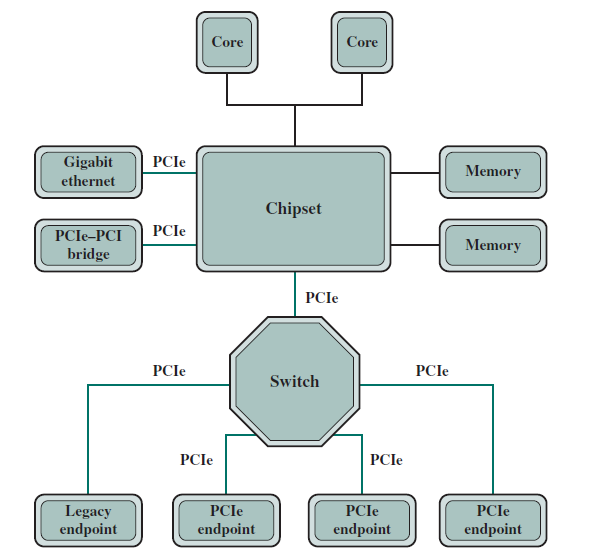
\includegraphics[width=\linewidth]{./Images/raiz.png}
\end{minipage}
\end{frame}

\begin{frame}[label={sec:org07014fc}]{Dispositivos que implementan PCIe}
\alert{\alert{Conmutador:}} El conmutador gestiona múltiples flujos PCIe.

\alert{\alert{Punto final PCIe:}} Dispositivo o controlador de E/S que implementa PCIe, como un
conmutador Gigabit ethernet, un controlador gráfico o de vídeo, una interfaz de
disco o un controlador de comunicaciones.

\alert{\alert{Endpoint heredado:}} La categoría de punto final heredado está pensada para diseños
existentes que se han migrado a PCI , y permite comportamientos heredados como uso de espacio de E/S y transacciones bloqueadas. No se permite que los
puntos finales PCI Express requieran el uso de espacio de E/S en tiempo de
ejecución y no deben utilizar transacciones bloqueadas.

\alert{\alert{Puente PCIe/PCI:}} Permite conectar dispositivos PCI antiguos a sistemas basados
en PCIe.
\end{frame}

\section{Arquitectura}
\label{sec:org53d85da}
\begin{frame}[label={sec:org3052cc1}]{La arquitectura del protocolo PCIe}
La arquitectura del protocolo PCIe abarca las siguientes capas:

\alert{\alert{Físico:}} Consiste en los propios cables que transportan las señales, así como los
circuitos y la lógica que soportan las funciones auxiliares necesarias en la
transmisión y recepción de los 1 y los 0.

\alert{\alert{Enlace de datos:}} Es responsable de la transmisión fiable y del control de flujo. Los
paquetes de datos generados y consumidos por la DLL se denominan paquetes de capa
de enlace de datos (DLLP).

\alert{\alert{Transacción:}} Genera y consume paquetes de datos utilizados para implementar
mecanismos de transferencia de datos de carga/almacenamiento y también gestiona
el control de flujo de dichos paquetes entre los dos componentes de un enlace. Los
paquetes de datos generados y consumidos por la TL se denominan paquetes de capa
de transacción (TLP).
\end{frame}

\begin{frame}[label={sec:org6e22a58}]{La arquitectura del protocolo PCIe}
\begin{center}
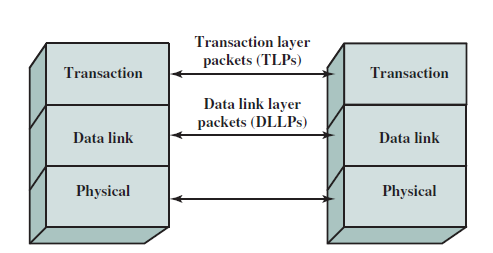
\includegraphics[width=.9\linewidth]{./Images/arquitectura.png}
\end{center}
\end{frame}

\section{Capas del Protocolo}
\label{sec:org811f028}
\begin{frame}[label={sec:org27b5e01}]{Capa Física}
La capa física de PCIe maneja la transmisión real de datos a través del medio físico. Emplea técnicas sofisticadas de codificación 128b/130b y scrambling para mantener la integridad de la señal y la sincronización. Estas técnicas permiten alcanzar velocidades de transferencia de hasta 16 GB/s, garantizando la fiabilidad en la transmisión de datos.
\end{frame}

\begin{frame}[label={sec:org5b1baf7}]{Capa de transacción PCIe}
La capa de transacciones (TL) recibe peticiones de lectura y escritura del software por
encima de la TL y crea paquetes de peticiones para su transmisión a un destino a través de
la capa de enlace. La mayoría de las transacciones utilizan una técnica de transacción
dividida. Con la técnica de
transacción dividida, la finalización está separada en el tiempo de la solicitud, en contraste
con una operación de bus típica en la que ambos lados de una transacción deben estar
disponibles para aprovechar y utilizar el bus. Entre la solicitud y la finalización, otro
tráfico PCIe puede utilizar el enlace.
\end{frame}

\begin{frame}[label={sec:org69e1ea7}]{Espacios de dirección}
La TL admite cuatro espacios de dirección:

\alert{\alert{Memoria:}} El espacio de memoria incluye la memoria principal del sistema.
También incluye los dispositivos de E/S PCIe. Ciertos rangos de direcciones de
memoria se asignan a dispositivos de E/S.

\alert{\alert{E/S:}} Este espacio de direcciones se utiliza para dispositivos PCI heredados, con
rangos de direcciones de memoria reservados utilizados para direccionar dispositivos
de E/S heredados.

\alert{\alert{Configuración:}} Este espacio de direcciones permite a la TL leer/escribir los registros de
configuración asociados a los dispositivos de E/S.

\alert{\alert{Mensaje:}} Este espacio de direcciones es para señales de control relacionadas con
interrupciones, manejo de errores y gestión de energía.
\end{frame}

\begin{frame}[label={sec:orgd21d508}]{Tipos de transmisión}
\begin{center}
\begin{tabular}{lll}
Espacio de direcciones & Tipo TLP & Propósito\\[0pt]
\hline
Memoria & Petición de lectura de memoria & Transfiere datos hacia o desde una ubicación en el mapa de memoria del sistema.\\[0pt]
 & Solicitud de bloqueo de lectura de memoria & \\[0pt]
 & Petición de escritura en memoria & \\[0pt]
\hline
E/S & Solicitud de lectura de E/S & Transfiere datos a o desde una ubicación en el mapa de memoria del sistema para dispositivos heredados.\\[0pt]
 & Solicitud de escritura de E/S & \\[0pt]
\hline
Configuración & Config Tipo 0 Petición de lectura & Transferir datos hacia o desde una ubicación en el espacio de configuración de un dispositivo PCIe.\\[0pt]
 & Config Tipo 0 Petición de escritura & \\[0pt]
 & Config Tipo 1 Petición de lectura & \\[0pt]
 & Solicitud de escritura Config Tipo 1 & \\[0pt]
\hline
Mensaje & Solicitud de mensaje & Proporciona mensajería en banda e informes de eventos.\\[0pt]
 & Solicitud de mensaje con datos & \\[0pt]
\hline
Memoria, E/S, Configuración & Finalización & Devuelto para determinadas solicitudes.\\[0pt]
 & Finalización con datos & \\[0pt]
 & Finalización bloqueada & \\[0pt]
 & Finalización bloqueada con datos & \\[0pt]
\end{tabular}
\end{center}
\end{frame}

\begin{frame}[label={sec:orgfdf432a}]{Formato de Unidad de Datos del Protocolo PCIe}
Las transacciones PCIe se transmiten utilizando paquetes de capa de transacción.
El formato de los paquetes en el protocolo PCIe (Peripheral Component Interconnect Express), desglosado en dos niveles:

1.- Paquete de la Capa de Transacción (Transaction Layer Packet - TLP):
Este paquete es generado por la capa de transacción y contiene las siguientes secciones:

\alert{\alert{STP framing (Start of TLP framing):}} Señal de inicio del paquete para delimitarlo. Ocupa 1 byte.

\alert{\alert{Sequence Number:}} Un campo que indica el número de secuencia del paquete para garantizar la entrega ordenada. También ocupa 1 byte.

\alert{\alert{Header:}} Contiene información esencial para procesar el paquete, como dirección, tipo de operación, etc. Puede ocupar 12 o 16 bytes, dependiendo de la operación.

\alert{\alert{Data:}} La carga útil del paquete, que puede variar entre 0 y 4096 bytes. Es opcional, dependiendo del tipo de transacción.

\alert{\alert{ECRC (End-to-End CRC):}} Código de redundancia cíclica (CRC) opcional para verificar la integridad de los datos de extremo a extremo. Ocupa 0 o 4 bytes.

\alert{\alert{LCRC (Link CRC):}} Otro CRC obligatorio para verificar la integridad de los datos en el enlace. También ocupa 4 bytes.

\alert{\alert{STP framing (End of TLP framing):}} Marca el final del paquete, similar al campo inicial.
Este paquete es luego entregado a la capa de enlace para mayor encapsulación.
\end{frame}

\begin{frame}[label={sec:org2600b64}]{Formato de Unidad de Datos del Protocolo PCIe}
2.-Paquete de la Capa de Enlace de Datos (Data Link Layer Packet - DLLP):
Este paquete es generado por la capa de enlace y es más pequeño que el TLP.

\alert{\alert{Start:}} Indica el inicio del paquete de la capa de enlace. Ocupa 1 byte.

\alert{\alert{DLLP:}} Contiene datos de control o gestión del enlace. Este es el núcleo del paquete de la capa de enlace.

\alert{\alert{CRC:}} Código de redundancia cíclica usado para verificar la integridad de los datos transmitidos. También ocupa 1 byte.

\alert{\alert{End:}} Indica el final del paquete. Ocupa 1 byte.
\end{frame}

\begin{frame}[label={sec:org162c825}]{Formato de Unidad de Datos del Protocolo PCIe}
\begin{center}
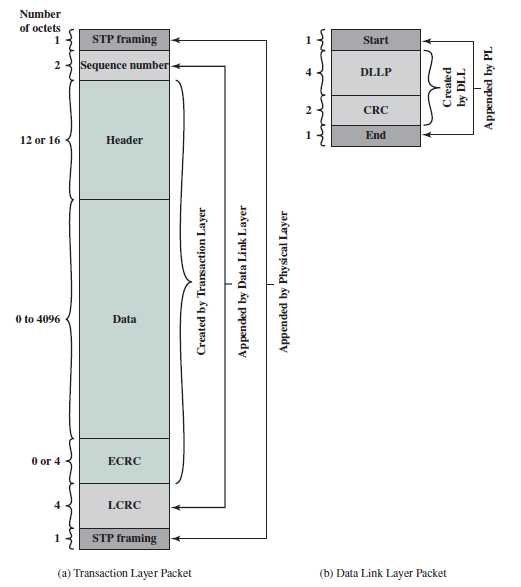
\includegraphics[width=.9\linewidth]{./Images/formato.png}
\end{center}
\end{frame}

\begin{frame}[label={sec:org6fa3c08}]{Capa de Enlace de Datos}
Esta capa implementa mecanismos robustos para garantizar la entrega confiable de datos. Gestiona el control de flujo y maneja los paquetes de nivel de enlace (DLLPs). Su sistema de verificación incluye números de secuencia y códigos de verificación, asegurando la integridad de cada transmisión.
\end{frame}



\section{Arquitectura PCIe}
\label{sec:orgc1da2bf}
\begin{frame}[label={sec:org4f61a57}]{Componentes Básicos}
\begin{itemize}
\item El sistema PCIe consta de varios componentes clave:
\begin{enumerate}
\item \alert{\alert{Root Complex}}: Es el componente principal que se conecta al procesador. Controla el acceso a los dispositivos y coordina las transferencias de datos.

\item \alert{\alert{Switches}}: Son los dispositivos que gestionan y dirigen el tráfico entre diferentes dispositivos conectados al sistema PCIe.

\item \alert{\alert{Endpoints}}: Son los dispositivos conectados al bus PCIe, como tarjetas gráficas, SSDs, y otros periféricos.
\end{enumerate}
\end{itemize}
\end{frame}

\section{Conclusiones}
\label{sec:org4232492}
\begin{frame}[label={sec:orge014e3d}]{Impacto en la Industria}
PCIe ha revolucionado la forma en que los componentes de computadora se comunican entre sí. Su arquitectura escalable y eficiente ha permitido el desarrollo de nuevas tecnologías y aplicaciones, estableciendo un estándar que continúa evolucionando para satisfacer las necesidades futuras de la industria.
\end{frame}


\section{Referencias}
\label{sec:org1dc2922}
\begin{frame}[allowframebreaks]{Bibliografía}
\printbibliography
\end{frame}
\end{document}
